\section[Overview]{Overview}
\subsection[Overview]{Overview}

\begin{frame}  \frametitle{Overview}
	\begin{itemize}
		\item Writing publications in team
		\item Counters
		\item Commands
		\item Environments
	\end{itemize}
\end{frame}

\section[Writing in Team]{Writing in Team}
\subsection[Writing in Team]{Writing in Team}

\begin{frame}  \frametitle{Challenages of writing in teams}

	\begin{itemize}	
		\item Scientific publications are written by group of people
		\item Different people are used to different software
		\item Publishers have their own standards and templates
		\item Never ending problem is a synchronization of changes
	\end{itemize}
\end{frame}


\begin{frame}  \frametitle{Using LaTeX for writing \textbf{team} publication}
	
	Common steps to be followed in order simplify writing publication in team.
	
	\vspace{0.4cm}
	
	
	\begin{itemize}	
		\item Separate content of the publication from it's processing part
		\item Make writing process transparent
		\begin{itemize}
			\item Host and share all the publication files through the dropbox or SVN
		\end{itemize}
		\item Organize versioning
		\begin{itemize}
			\item Default feature of documents hosting services like dropbox and SVN
		\end{itemize}
		\item Separate part of each author into different TeX file or files
		\begin{itemize}
			\item Include them with {\color{command}$\backslash$input\color{braces}$\{${\color{black}fileName}$\}$\color{black}} directive
		\end{itemize}
	\end{itemize}
\end{frame}


\begin{frame}  \frametitle{Organizing your folder}
	
	An example how folder with all relevant to publication files can be organized.
	
	\begin{columns}
		\column{0.5\textwidth} %half slide's text width
		\begin{itemize}
			\item \textbf{abstract}
				\begin{itemize}
					\item contains abstract part of the publication
				\end{itemize}
			\item \textbf{authors}
				\begin{itemize}
					\item contains authors listed with accordance to the template
				\end{itemize}					
			\item \textbf{bibliography}
			\begin{itemize}
				\item contains a BibTeX file with all cited works
			\end{itemize}					
			\item \textbf{models}
			\begin{itemize}					
				\item contains the images, diagrams etc.
			\end{itemize}					
		\end{itemize}

		\column{0.5\textwidth} %half slide's text width
			\begin{center}
				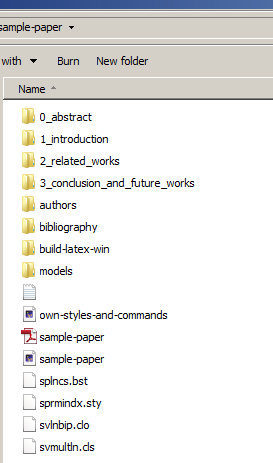
\includegraphics[height=2.2in]{tips/images/sampleFolderStructure}
			\end{center}
	\end{columns}
		

	
\end{frame}

\begin{frame}  \frametitle{Organizing your main TeX file}
	
	An example how main TeX file that actually contains only references to content in other TeX files can be organized.
	
	\vspace{0.2cm}
	
	\begin{center}
		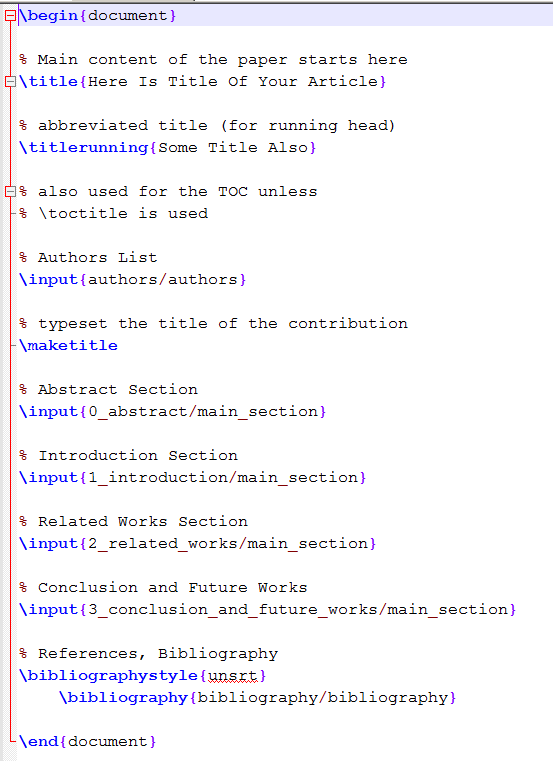
\includegraphics[height=2.4in]{tips/images/sampleMainTeXFile}
	\end{center}
	
\end{frame}





\section[Counters]{Counters}
\subsection[Counters]{Counters}

\begin{frame}  \frametitle{Existing counters}
	LaTeX uses counters (variables) to keep proper numbering. 
	\begin{itemize}
		\item The following are counters used by LaTeX: \texttt{\color{highlight}part}, \texttt{\color{highlight}chapter}, \texttt{\color{highlight}section}, \texttt{\color{highlight}subsection}, \texttt{\color{highlight}subsubsection}, \texttt{\color{highlight}page}, \texttt{\color{highlight}footnote}, \texttt{\color{highlight}equation}, \texttt{\color{highlight}figure}, and \texttt{\color{highlight}table}. These counters correspond to their corresponding commands.
		\item Other counters are used for each level of enumerate: \texttt{\color{highlight}enumi}, \texttt{\color{highlight}enumii}, \texttt{\color{highlight}enumiii}, \texttt{\color{highlight}enumiv}.
		\item A few other LaTeX counters: \texttt{\color{highlight}paragraph}, \texttt{\color{highlight}subparagraph}, \texttt{\color{highlight}mpfootnote}.
	\end{itemize}
\end{frame}

\begin{frame}  \frametitle{Create new counters}
	We may want to create our own counters for our own purposes. Maybe we have examples that we want numbered.
	\begin{itemize}
		\item[] {\color{command}$\backslash$newcounter\color{braces}$\{${\color{black}counterName}$\}$\color{black}[inCounter]}
	\end{itemize}
	This creates a new counter called \texttt{counterName}. The \texttt{inCounter} argument $+$ brackets are optional and an \texttt{inCounter} is used to reset \texttt{counterName} whenever \texttt{inCounter} increments (e.g. \texttt{subsection} has ``inCounter'' \texttt{section}).
\end{frame}

\begin{frame}  \frametitle{Modifying}
	We can modify existing or new counters.
	\begin{itemize}
		\item[] {\color{command}$\backslash$setcounter\color{braces}$\{${\color{black}counter}$\}\{${\color{black}n}$\}$}
		\item[] {\color{command}$\backslash$addtocounter\color{braces}$\{${\color{black}counter}$\}\{${\color{black}n}$\}$}
		\item[] {\color{command}$\backslash$stepcounter\color{braces}$\{${\color{black}counter}$\}$}
		\item[] {\color{command}$\backslash$refstepcounter\color{braces}$\{${\color{black}counter}$\}$}
	\end{itemize}
	The {\color{command}$\backslash$refstepcounter} command lets us reference our counter value if we follow it with a {\color{command}$\backslash$label}.
\end{frame}

\begin{frame}  \frametitle{Printing}
	So we can create, modify, and reference counters. However, we also need to print counters in the document. We do so by calling the counter with one of the following commands:
	\newcounter{temp}
	\setcounter{temp}{4}
	\begin{itemize}
		\item[] {\color{command}$\backslash$arabic}{\color{braces}$\{${\color{black}chapter}$\}$} (\arabic{temp}, Arabic number)
		\item[] {\color{command}$\backslash$Roman} (\Roman{temp}, uppercase Roman numeral)
		\item[] {\color{command}$\backslash$roman} (\roman{temp}, lowercase Roman numeral)
		\item[] {\color{command}$\backslash$Alph} (\Alph{temp}, capital letter)
		\item[] {\color{command}$\backslash$alph} (\alph{temp}, lowercase letter)
		\item[] {\color{command}$\backslash$fnsymbol} (\fnsymbol{temp}, footnote symbol)
	\end{itemize}
	We will put counters to use in our custom commands and environments.
\end{frame}

\section[Commands]{Commands}
\subsection[Commands]{Commands}

\begin{frame}  \frametitle{Simple command}
	\newcommand{\xvec}{x_1, \ldots, x_n}
	Common statements, like $x_1, ..., x_n$ can be abbreviated using a new command.
	\begin{itemize}
		\item[] {\color{command}$\backslash$newcommand\color{braces}$\{${\color{command}$\backslash$xvec}$\}\{${\color{black}x\_1,{\color{command}$\backslash$dots},x\_n}$\}$}
	\end{itemize}
	Inserting this command and then typing (later in the document) {\color{braces}\$\color{command}$\backslash$xvec\color{braces}\$}, we get $\xvec$. If we forgot the dollar signs, we would be in trouble. We can resolve this by using an extra command:
	\begin{itemize}
		\item[] {\color{command}$\backslash$newcommand\color{braces}$\{${\color{command}$\backslash$xvec}$\}\{${\color{command}$\backslash$ensuremath{\color{braces}$\{$}{\color{black}x\_1,{\color{command}$\backslash$dots},x\_n}}$\}$ $\}$}
	\end{itemize}
	In the second definition, we left an extra space at the end, which helps prevent spacing problems. More elegant solution is to use the {\color{highlight}xspace} package (see \textit{Guide to LaTeX}, page 186).
\end{frame}

\newcommand{\subvec}[2]{\ensuremath{#1_{1}, \ldots, #1_{#2}} }
\begin{frame}  \frametitle{Command with arguments}
	If we want to generalize our command, we add two arguments
	\begin{itemize}
		\item[] \hspace{-1mm}{\color{command}$\backslash$newcommand\color{braces}$\{${\color{command}$\backslash$subvec}$\}${\color{black}[2]}$\{${\color{command}$\backslash$ensuremath{\color{braces}$\{$}{\color{black}\#1\_1,{\color{command}$\backslash$dots},\#1\_{\color{braces}$\{$}\#2{\color{braces}$\}$}}}$\}$ $\}$}
	\end{itemize}
	We can create \subvec{y}{m} from {\color{command}$\backslash$subvec\color{braces}$\{${\color{black}y}$\}\{${\color{black}m}$\}$}.
	
	\vspace{7mm}
	
	Additional arguments can be created and are referenced via \#n for the $n^{th}$ argument. Optional default arguments can also be utilized (see \textit{Guide to LaTeX}, page 188).
\end{frame}

\begin{frame}  \frametitle{Generalization}
	The general framework of new commands is
	\vspace{0.5mm} \\
	\begin{itemize}
		\item[] {\color{command}$\backslash$newcommand\color{braces}$\{${\color{command}$\backslash$commandName}$\}${\color{black}[n]}$\{${\color{highlight}the commands}$\}$}
	\end{itemize}
	\vspace{0.5mm}
	where
	\vspace{0.5mm} \\
	\begin{itemize}
		\item \texttt{commandName} is the name of the command,
		\item \texttt{n} is the number of arguments, and
		\item the arguments are referred to as \#1, \#2, \dots, \#n in {\color{highlight}the commands}.
	\end{itemize}
	\vspace{0.5mm}
	To redefine a command that already exists, use {\color{command}$\backslash$renewcommand} with the same format as above.
\end{frame}

\section[Environments]{Environments}
\subsection[Environments]{Environments}

\begin{frame}  \frametitle{Sample environment}
	Environments use begin and end tags (e.g. \texttt{itemize}). We only need define what happens at the {\color{command}$\backslash$begin} and {\color{command}$\backslash$end} tags. For example,
	\begin{itemize}
		\item[] {\color{command}$\backslash$newenvironment\color{braces}$\{${\color{black}example}$\}$}
		\item[] \hspace{2mm}{\color{braces}$\{${\color{command}$\backslash$small$\backslash$textbf}$\{${\color{black}Example.}$\}$ {\color{command}$\backslash$hspace}$\{${\color{black}2mm}$\}\}$ {\color{red}\% begin stuff}}
		\item[] \hspace{2mm}{\color{braces}$\{${\color{command}$\backslash\backslash$}$\}$ {\color{red}\% end stuff}}
	\end{itemize}
	Sample environment call:
	\begin{itemize}
		\item[] {\color{command}$\backslash$begin\color{braces}$\{${\color{black}example}$\}$}
		\item[] Modular addition works in mysterious ways: {\color{braces}\$}2+2=1{\color{braces}\$} (mod 3).
		\item[] {\color{command}$\backslash$end\color{braces}$\{${\color{black}example}$\}$}
	\end{itemize}
	Result:
	\vspace{5mm} \\
	\small\textbf{Example.}\hspace{1.5mm} Modular addition works in mysterious ways: $2+2 = 1$ (mod 3).
\end{frame}

\begin{frame}  \frametitle{General environment}
	Generally environments take the form
	\vspace{0.5mm} \\
	\begin{itemize}
		\item[] {\color{command}$\backslash$newenvironment\color{braces}$\{${\color{black}environmentName}$\}\{${\color{highlight}begin stuff}$\}\{${\color{highlight}end stuff}$\}$}
	\end{itemize}
	\vspace{0.5mm}
	We can also declare that there will be \texttt{n} arguments.
	\vspace{0.5mm} \\
	\begin{itemize}
		\item[] {\color{command}$\backslash$newenvironment\color{braces}$\{${\color{black}environmentName}$\}${\color{black}[n]}$\{${\color{highlight}begin stuff}$\}\{${\color{highlight}end stuff}$\}$}
	\end{itemize}
	\vspace{0.5mm}
	As before, we refer to the arguments as \#1, \dots, \#n in the {\color{highlight}begin stuff} and {\color{highlight}end stuff}.
	\vspace{7mm} \\
	To redefine an environment that already exists, use {\color{command}$\backslash$renewenvironment} with the same format as above.
\end{frame}

\begin{frame}  \frametitle{Environment + counter}
	\begin{itemize}
		\item[] {\color{command}$\backslash$newcounter\color{braces}$\{${\color{black}example}$\}$}
		\item[] {\color{command}$\backslash$setcounter\color{braces}$\{${\color{black}example}$\}$$\{${\color{black}0}$\}$}
		\item[] {\color{command}$\backslash$newenvironment\color{braces}$\{${\color{black}example}$\}$}
		\item[] \hspace{4mm}{\color{braces}$\{${\color{command}$\backslash$refstepcounter\color{braces}$\{${\color{black}example}$\}$}\color{command}$\backslash$small}
		\item[] \hspace{8mm}{\color{braces}{\color{command}$\backslash$textbf}$\{${\color{black}Example} {\color{command}$\backslash$arabic\color{braces}$\{${\color{black}example}$\}$}{\color{black}.}$\}${\color{command}$\backslash$hspace}$\{${\color{black}2mm}$\}\}$}
		\item[] \hspace{4mm}{\color{braces}$\{${\color{command}$\backslash\backslash$}$\}$}
	\end{itemize}
\end{frame}


